% !TEX root = main.tex

\section{Path explosion}
\label{se:path-explosion}

One of the main challenges of symbolic execution is the path explosion problem. As symbolic execution may fork off a new execution engine instance at every branch, the total number of executors may be exponential in the number of branches in the program. This impacts both time and space, since a symbolic executor may need to keep track of an exponential number of pending branches to be explored. A common approach is to compute an under-approximation of the analysis that only explores a relevant subset of the state space.
%\mynote{I: We could add the following two examples to explain the causes of path explosion (Vechev)}

Loops are one of the main causes of path explosion: each iteration of a loop can be seen as an {\tt if-goto} statement, leading to a conditional branch in the execution tree. If the loop condition involves one or more symbolic values, the number of generated branches may be potentially infinite. 

\begin{figure}[t]
\begin{center}
\begin{tabular}{c}
\begin{lstlisting}[basicstyle=\ttfamily\scriptsize]
1.  int x = sym_input(); // e.g., read from file
2.  while (x > 0) {
3.     x = sym_input();  
4.  }
\end{lstlisting}
\end{tabular}
\end{center}
\vspace{-2mm}
\caption{Loop example with input read from the environment~\protect\cite{CS-CACM13}.}
\label{fi:example-loop}
\end{figure}

\vspace{-2pt} % TODO
\boxedexample{Consider the code fragment of Figure~\ref{fi:example-loop}~\cite{CS-CACM13}, where \texttt{sym\_input()} is an external routine that interacts with the environment (e.g., by reading input data from a network) and returns a fresh symbolic input. The path constraint set at any final state has the form: 
\[ \pi = \left ( \bigwedge_{i \in [1, k]} \alpha_i > 0 \right ) \wedge (\alpha_{k+1} \leq 0) \] 
where $k$ is the number of iterations and $\alpha_i$ is the symbol produced by \texttt{sym\_input()} at the $i$-th iteration.}



\iffalse
\begin{itemize}

\item Exponential in branching structure: in the example, 3 variables, 8 paths (can we generalize? $t$ variables, $2^t$ paths?)

\begin{verbatim}
1. int a = ?, b = ?, c = ?; // symbolic
2. if (a) ... else ...;
3. if (b) ... else ...;
4. if (c) ... else ...;
\end{verbatim}

\item Loops on symbolic variables even worse

\begin{verbatim}
1. int a = ?; // symbolic
2. while (a) do ...;
3.
\end{verbatim}
\item Potentially $2^{31}$ paths through loop!

\end{itemize}
\fi

\begin{figure}[t]
  \centering
  \begin{adjustbox}{width=0.84\columnwidth} % TODO was 1; with 0.88 the last paragraph will fit
  \begin{small}
  \begin{tabular}{| l || l |}
    \hline      
    {\bf Heuristic} & {\bf Goal} \\ \hline\hline
    \multirow{2}*{BFS} & {\em Maximize coverage} \\ & \cite{CKC-TOCS12,PEX-TAP08} \\\hline
    \multirow{3}*{DFS} & {\em Exhaust paths, minimize memory usage} \\ & \cite{EXE-CCS06,CKC-TOCS12}\\ & \cite{PEX-TAP08,DART-PLDI05} \\\hline
    \multirow{2}*{Random path selection} & {\em Randomly pick a path with probability based on its length} \\ & \cite{KLEE-OSDI08} \\\hline
    %low-covered code & prioritize paths that execute low-covered code  & \cite{EXE-CCS06} \\
    \multirow{3}*{Code coverage search} & {\em Prioritize paths that may explore unexplored code} \\ & \cite{EXE-CCS06,KLEE-OSDI08,MAYHEM-SP12}\\ & \cite{CKC-TOCS12,GV-ISSTA02} \\\hline
    \multirow{2}*{Buggy-path-first} & {\em Prioritize bug-friendly path} \\ & \cite{AEG-NDSS11} \\\hline
    \multirow{2}*{Loop exhaustion} & {\em Fully explore specific loops} \\ & \cite{AEG-NDSS11} \\\hline
    \multirow{2}*{Symbolic instruction pointers} & {\em Prioritize paths with symbolic instruction pointers} \\ & \cite{MAYHEM-SP12} \\\hline
    \multirow{2}*{Symbolic memory accesses} & {\em Prioritize paths with symbolic memory accesses} \\ & \cite{MAYHEM-SP12} \\ \hline
    \multirow{2}*{Fitness function} & {\em Prioritize paths based on a fitness function} \\ & \cite{XTD-DSN09,CS-CACM13,XTD-DSN09} \\ \hline
    \multirow{3}*{Subpath-guided search} & {\em Use frequency distributions of explored subpaths to prioritize}\\ & {\em less covered parts of a program} \\ & \cite{LZL-OOPSLA13} \\
    %kill path & filter uninteresting path & \cite{CKC-TOCS12} \\
    \hline  
  \end{tabular}
  \end{small}
  \end{adjustbox}
  \caption{Common path selection heuristics discussed in literature.}
  \label{tab:heuristics}
\end{figure}


% ---------------------------------------------------------------------------------------------------
\subsection{Path Selection}
\label{ss:heuristics}

\mytempedit{
\myedit{Another} common approach is to limit the amount of resources symbolic execution is allowed to use. For instance, the computation may time out after a certain amount of time. Since only a fraction of paths may be explored, the search should be prioritized by looking at the most promising paths first. There are several strategies for selecting or generating the next path to be explored. We now briefly overview some of the most interesting techniques that have been shown to be effective in the literature. %in prior works.
}
%\subsubsection{Search Heuristics}
%\label{sss:search-heuristics}

% many prior works
%\myparagraph{Search Heuristics} 
Given a set of unexplored paths, a search heuristic should select the most promising path to explore. Many works have introduced novel search strategies, showing their effectiveness in specific application contexts. These heuristics have often been tailored to help the symbolic engine achieve a specific goal (e.g., overflow detection). Finding a universally optimal strategy for prioritizing path exploration remains an open problem. Table~\ref{tab:heuristics} provides a sample of prominent search heuristics discussed in prior works. 

The most common strategies are {\em depth-first search} (DFS) and {\em breadth-first search} (BFS). DFS continuously expands a path as much as possible, before backtracking to the deepest unexplored branch. BFS explores all unexplored paths in parallel, repeatedly expanding each of them by a fixed slice. DFS is often adopted for minimizing the memory usage of the symbolic engine: since the chosen path will be sooner or later fully explored, the memory needed for keeping its state will be released as well. Unfortunately, paths containing loops and recursive calls can easily stall the symbolic engine. For this reason, some tools prefer prioritizing paths using BFS. Although memory pressure can be higher, this strategy may allow an engine to quickly explore diverse paths and possibly detecting interesting behaviors. \iffullver{On the other hand, if the ultimate goal requires to fully terminate the exploration of one or more paths, BFS may take a very long time}{However, if the ultimate goal requires to fully terminate the exploration of one or more paths, BFS may take a very long time}.

Another popular strategy is {\em random path selection} that, as its name would suggest, randomly picks a path for exploration. This heuristic has been refined in several variants. For instance, {\sc KLEE}~\cite{KLEE-OSDI08} assigns probabilities to paths based on their length and on the branch arity. Namely, it favors paths that have been explored fewer times, preventing starvation caused by loops and other path explosion factors.

% have instead presented
Several works, such as {\sc EXE}~\cite{EXE-CCS06}, {\sc KLEE}~\cite{KLEE-OSDI08}, {\sc Mayhem}~\cite{MAYHEM-SP12}, and {\sc \stwoe}~\cite{CKC-TOCS12}, have discussed heuristics aimed at maximizing code coverage. For instance, the {\em coverage optimize search} discussed in {\sc KLEE}~\cite{KLEE-OSDI08} computes for each state a weight, which is later used to randomly select states. The weight is obtained by considering how far the nearest uncovered instruction is, whether new code was recently covered by the state, and the state's call stack. Of a similar flavor is the heuristic proposed in~\cite{LZL-OOPSLA13}, called {\em subpath-guided search}, which attempts to explore {\it less traveled} parts of a program by selecting the subpath of the control flow graph that has been explored fewer times. This is achieved by maintaining a frequency distribution of explored subpaths, where a subpath is defined as a consecutive subsequence of length $n$ from a complete path. Interestingly, the value $n$ plays a crucial role with respect to the code coverage achieved by a symbolic engine using this heuristic and no specific value has been shown to be universally optimal.

Other search heuristics try to prioritize paths likely leading to states that are {\em interesting} according to some goal. For instance, the {\em buggy-path first} strategy in {\sc AEG}~\cite{AEG-NDSS11} picks paths whose past states have contained small but unexploitable bugs. The intuition is that if a path contains some small errors, it is likely that it has not been properly tested. There is thus a good chance that future states may contain interesting, and hopefully exploitable, bugs. Similarly, the {\em loop exhaustion} strategy discussed in {\sc AEG}~\cite{AEG-NDSS11} explores paths that visit loops. This approach is inspired by the practical observation that common programming mistakes in loops may lead to buffer overflows or other memory-related errors. In order to find exploitable bugs, {\sc Mayhem}~\cite{MAYHEM-SP12} instead gives priority to paths where symbolic memory accesses are identified or symbolic instruction pointers are detected. 

{\em Fitness functions} have been largely used in the context of search-based test generation~\cite{M-STVR04}. %\mynote{[D] Check and rephrase 2nd sentence}
A fitness function measures how close an explored path is to achieve the target test coverage. Several papers, e.g.,~\cite{XTD-DSN09,CS-CACM13,XTD-DSN09}, have applied this idea in the context of symbolic execution. As an example,~\cite{XTD-DSN09} introduces {\em fitnex}, a strategy for concolic execution that prioritizes paths that are {\em closer} to take a specific branch. In more detail, given a branch condition of the form $|a - c| == 0$ and a path that has reached the branch, {\em fitnex} computes a closeness equal to $|a - c|$ by leveraging the concrete values \iffullver{of the two}{of} variables $a$ and $c$ in that path. Similar fitness values can be computed for other kinds of branch conditions. The path with the lowest fitness value for a branch is selected by the symbolic engine. Paths that have not reached the branch yet get the worst-case fitness value.

% ---------------------------------------------------------------------------------------------------
\subsection{Pruning Unrealizable Paths}
\label{ss:unrealizable-paths}

\begin{figure}[t]
  %\vspace{-3mm}
  %\centering
  \begin{subfigure}{.29\textwidth}
    \vspace{0mm}
    \begin{lstlisting}[basicstyle=\ttfamily\scriptsize]
   if (a > 0) {
      ...
   } 

   if (a > 1) {
      ...
   }
    \end{lstlisting}
    \vspace{-0.7mm}
    \caption{}
  \end{subfigure}%
  %\hspace{-2mm}
  \begin{subfigure}{.70\textwidth}
    \centering
    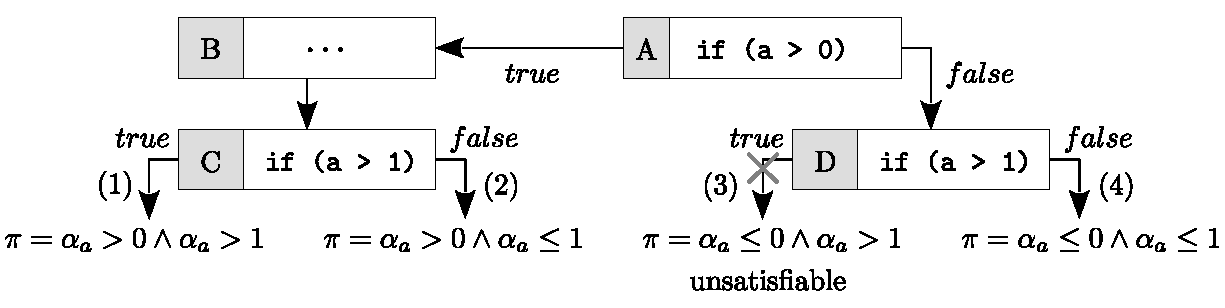
\includegraphics[width=1.0\columnwidth]{images/eager-evaluation} 
    %\label{fig:sub1}
    \vspace{-5mm}
    \caption{}
  \end{subfigure}%
  \vspace{-2mm}
  \caption{Pruning unrealizable paths example: (a) Fragment of code; (b) Symbolic execution of the \iffullver{fragment of code}{code}: the {\em true} branch in node D is not explored since its path constraints $(\alpha_a \leq 0 \wedge \alpha_a > 1)$ are not satisfiable, i.e., there exists no assignment of variable {\tt a} that can drive a concrete execution first toward node D and then through its {\em true} branch.}
  \label{fig:eager-evaluation}
\end{figure}

\myedit{A first natural technique} for reducing the path space is invoking the constraint solver at each branch, pruning branches that are not realizable. Indeed, if the constraint solver is able to prove that the logical formula given by the path constraints of a branch is not satisfiable, then there exists no assignment of the program input values that would drive a real execution toward that path. For this reason, the symbolic engine can safely discard the path involving that branch without affecting soundness of the approach. 

\boxedexample{Consider the example shown in Figure~\ref{fig:eager-evaluation}. Assuming that {\tt a} is a local variable bound to an unconstrained symbol $\alpha_a$, a symbolic engine would start the execution of the code fragment in Figure~\ref{fig:eager-evaluation}a by evaluating the branch condition $a > 0$. Before expanding both branches, the symbolic engine queries a constraint solver to verify that no contradiction arises when adding to the path constraints $\pi$ the {\em true} branch condition ($\alpha_a > 0$) or the {\em false} branch condition ($\alpha_a \leq 0$). Since both paths are feasible, the engine forks the execution states B and D (Figure~\ref{fig:eager-evaluation}b). A similar scenario happens when the engine evaluates the branch condition $a > 1$. However, since $\alpha_a$ is not unconstrained anymore, some contradictions may be actually possible. The engine queries the solver to check the following path constraints: (1) $\alpha_a > 0~\wedge~\alpha_a > 1$, (2)~$\alpha_a > 0~\wedge~\alpha_a \leq 1$, (3) $\alpha_a \leq 0~\wedge~\alpha_a > 1$, and (4) $\alpha_a \leq 0~\wedge~\alpha_a \leq 1$. Notice that formula $\alpha_a \leq 0 \wedge \alpha_a > 1$ does not admit a valid solution and thus the related path can be safely dropped by the engine since it is unrealizable. On the other hand, other paths admit a valid solution and can be further explored by the engine.}

\noindent This approach is commonly referred as {\em eager evaluation} of path constraints since path constraints are eagerly checked at each branch and is typically the default approach adopted by most symbolic engines. We refer to Section~\ref{se:constraint-solving} for a discussion of the possible benefits given by the opposite strategy, i.e., {\em lazy evaluation}, where path constraints are lazily checked in order to possibly reduce the burden on the solver.

% From warm-up example\mynote{IF: I removed from the warm up the non-forking case. Must be explained here}:

% The evaluation of a conditional branch ${\tt if}~e~{\tt then}~s_{true}~{\tt else}~s_{false}$ affects the path constraint. Two scenarios are possible:
%     \begin{enumerate}
%       \item {\em Non-forking}: if $e$ is evaluated as always true (resp., false) under the assumptions in the current state, the proper branch is taken and the symbolic execution advances to $s_{true}$ (resp., $s_{false}$);
%       \item {\em Forking}: if $e$ cannot be evaluated without instantiating values for one or more of its symbols, the symbolic execution is forked by creating two execution states with path constraints $pct_{true}$ and $pct_{false}$, respectively, corresponding to the two {\tt if} branches. Namely, $pct_{true}=pct \wedge e_s$ and $pct_{false}=pct \wedge \neg e_s$, where $e_s$ is a symbolic expression obtained by evaluating $e$. 
% %        \[ (s_{true}, pc_{true}) \text{ where } pc_{true} = pc \wedge e \]
% %        \[ (s_{false}, pc_{false}) \text{ where } pc_{false} = pc \wedge \neg e \]
%     Symbolic execution proceeds on both states in parallel.
%     \end{enumerate}

\subsection{Function calls} 
\label{ss:functions}

\mytempedit{Function calls and loops are the main sources of path explosion in symbolic execution. Many works have attempted to capture similarities across distinct function invocations or loop iterations by devising {\em summarization} strategies for the effects of a computation so to prevent repeated explorations of a code portion, or by inferring {\em invariants} that describe properties of a computation inductively. In this section we present a number of prominent techniques appeared in the symbolic execution literature for handling function calls, and discuss connections with other program analysis and verification techniques. Loops are treated separately in the next section.}

A function $f$, and more in general any part of a program, may be called multiple times during an execution, either at the same calling context or at different ones. The traditional symbolic execution approach requires to symbolically execute $f$ at each call. \cite{G-POPL07} proposes a compositional approach that dynamically generates {\em function summaries}, allowing the symbolic executor to effectively reuse prior discovered analysis results. \mytempedit{Proposed for concolic executors, the technique captures the effects of a function invocation with a formula $\phi_w$ conjoining constraints on the inputs, which describe equivalence classes of concrete executions, with constraints observed on the output. A function summary then becomes a propositional logic formula defined as the disjunction of $\phi_w$ formulas from distinct classes.}

\mynote{TODO: Add paper read by Emilio}
A similar idea has been also proposed in~\cite{BCE-TACAS08}. The main intuition is that, if two program states differ only for some program values that are not read later, the executions generated by the two program states will produce the same side effects. Side effects of a portion of code can be therefore cached and possibly reused later.

% proved to be weak
% is a static checker based on verification conditions (i.e., logical formulas capturing correctness properties in a program) that
\mytempedit{Function summaries have largely been employed in static and dynamic program analysis techniques, especially in program verification. A number of such works offer interesting opportunities to advance the state of the art in symbolic execution. For instance, the Calysto static checker~\cite{CALYSTO-ICSE08} walks the call graph of a program to construct a symbolic representation of the effects of each function, i.e., return values, writes to global variables, and memory locations accessed depending on its arguments. Each function is processed once, possibly inlining effects of small ones at their call sites. Static checkers such as Calysto~\cite{CALYSTO-ICSE08} and Saturn~\cite{SATURN-POPL05} trade scalability for soundness in summary construction, as they unwind loops only to a small number of iterations: such techniques could then only be used for loop-free functions in the symbolic execution setting. More fine-grained summaries are constructed in~\cite{RACERX-SOSP03} by taking into account different input conditions using a summary cache for memoizing the effects of a function.

\cite{SFS11} proposes a technique to extract function summaries for model checking where multiple specifications are typically checked one a time, so that summaries can be reused across verification runs. In particular, they are computed as over-approximations using interpolation -- a technique that we discuss in detail in Section~\ref{ss:interpolation} -- and refined across runs when too weak. The strength of this technique lies in the fact that an interpolant-based summary can capture all the possible execution traces through a function in a more compact way than the function itself. The technique has later been extended to deal with nested function calls in~\cite{SFS12}, which discusses an useful application in incremental update checking of programs. 
}

\subsection{Loops} 
\label{ss:loops}

The problem of path explosion due to symbolic execution of loops has been attacked from different sides. \mytempedit{In this section we review the main approaches in the literature, and explore connections with other program analysis and verification techniques.}

\mytempedit{\myparagraph{Bounded Exploration}}
A first natural strategy adopted by many symbolic engines is to limit the loop exploration up to a certain number of iterations. Obviously, this may lead to missing interesting paths in the program. For this reason, some works (e.g., {\sc AEG}~\cite{AEG-NDSS11}) have also considered the opposite strategy, allowing the engine to fully explore some loops. To mitigate the path explosion problem, only a single instance of the symbolic executor is allowed to fully unroll a loop, while other instances conservatively explore other paths. This approach has been shown to be effective in some application contexts such as security (e.g., identification of buffer overflows) where interesting behavior may be observed at the loop boundaries.

By using static or dynamic analysis techniques, it may be possible to derive properties over a loop that can be exploited by the symbolic engine to significantly prune branching paths. For instance, knowledge of the exact number of loop iterations - or at least a constant upper bound on it - can significantly help the engine. Section~\ref{precontioned-symbolic-execution} provides a more general discussion of how preconditions can help symbolic execution.

\mytempedit{\myparagraph{Summaries}}
\cite{GL-ISSTA11} presents a technique that automatically derives partial summarizations for loops. A loop summarization is similar to a function summary, using a set of preconditions and a set of postconditions. These are computed dynamically during the symbolic execution by reasoning on the dependencies among loop conditions and symbolic variables. As soon as a loop summary is computed, it is cached for possibly subsequent reuse. This not only allows the symbolic engine to avoid redundant executions of the same loop under the same program state, but also makes it possible to generalize the loop summary to cover even different executions of the same loop that run under different conditions. A main limitation of this approach is that it can generate summaries only for loops that iteratively update symbolic variables across loop iterations by adding a constant, non-zero amount.

\mytempedit{
  % still WIP
 \myedit{Another} crucial limitation of \myedit{early summarization} works is that in general they cannot handle nested loops as well as {\em multi-path loops}, i.e., loops that contain one or more branches. In the last few years, the latter scenario has been effectively tackled first by S-Looper~\cite{XX-ISSTA15} and later by Proteus~\cite{XX-FSE16}. S-Looper targets loops that traverse a string, without modifying it, and that have branch conditions related to the traversed string or other loop induction variables. Proteus has made a step further by proposing a more general framework for summarization of multi-path loops. First, it classifies loops based on the patterns of value changes, i.e., whether the loop variables are induction or non-induction, and based on the patterns of path interleaving, i.e., whether the path interleaving can be considered {\em sequential}, {\em periodic}, or {\em irregular}. In order to perform loop classification, Proteus constructs a flowgraph of the sliced loop program. Loop slicing is performed exploiting the program dependence graph (PDG), which combines the control flow graph (CGF) and the data dependencies of the loop. The flowgraph is then analyzed and the loop classified. Depending of the type of the loop, different strategies are used for generating a disjunctive loop summarization (DLS). Intuitively, a DLS is the union of all the trace summaries for a loop. For instance, loops that contain only induction variables and that have a path interleaving with a periodic pattern are summarized by first constructing the path dependency automaton (PDA) of the loop, then by summarizing the effect of distinct paths (periods) of the cycle and finally by relating these effects to the execution number of the loop. Although not all types of loops can be summarized by Proteus, it still can produce approximated loop summaries for many different types, which could be useful in practice. Precise summarization of multi-path loops with non-induction variables or with an irregular pattern, or even worse summarization of nested loops, still remain an open research problem. 
}

\mytempedit{\myparagraph{Invariants}
Loop invariants play a key role in verifiers that can prove programs correct against their full functional specification. An invariant is not just a quantity that remains unchanged throughout executions of the loop body, but an inductive property that holds when the loop is first entered and is preserved for an arbitrary number of iterations~\cite{FMV-CSUR14,GFM-TSE15}. Leveraging invariants can be beneficial to symbolic executors, in order to compactly capture the effects of a loop and reason about them. Unfortunately, we are not aware of symbolic executors taking advantage of this approach. One of the reasons might lie in the difficulty of computing loop invariants without requiring manual intervention from domain experts. In fact, lessons from the verification practice suggest that providing loop invariants is much harder compared to other specification elements such as method pre/post-conditions.

% a number of works [...] and might be
However, many researchers have recently explored techniques for inferring loop invariants automatically or with little human help~\cite{FMV-CSUR14}, which might be of interest for the symbolic execution community.
%
% that rank all -> over all
{\em Termination analysis} has been applied to verify program termination for industrial code: a formal argument is typically built by using one or more ranking functions over all the possible states in the program such that for every state transition, at least one function decreases~\cite{CPR-PLDI06}. Ranking functions can be constructed in a number of ways, e.g., by lazily building an invariant using counterexamples from traversed loop paths~\cite{GMR-PLDI15}. Another way to construct a termination argument is to reason over loop-free code by using loop summaries based on transition invariants~\cite{TSW-TACAS11}. It has been observed that most loops in practice have relatively simple termination arguments~\cite{TSW-TACAS11}, and discovered invariants may thus be too simple for a verification setting~\cite{GFM-TSE15}. However, a constant or parametric bound on the number of iterations may be computed from a ranking function and an invariant~\cite{GMR-PLDI15}.
%
{\em Predicate abstraction} is as a form of abstract interpretation over a domain constructed using a given set of predicates, and has been used to infer universally quantified loop invariants~\cite{FQ-POPL02}, which are useful when manipulating arrays. Predicates can be heuristically collected from the code or supplied by the user; it would be interesting to explore whether an executor might provide useful predicates from a symbolic exploration of the code. {\em LoopFrog}~\cite{LOOPFROG-ATVA08} replaces loops using a symbolic abstract transformer with respect to a set of abstract domains, obtaining a conservative abstraction of the original code. Abstract transformers are computed starting from the innermost loop, and the output is a loop-free summary of the program that can be handed to a model checker for verification. This approach can also be applied to non-recursive function calls, and might deserve further investigation in symbolic executors. Loop invariants can also be extracted using {\em interpolation}, a general technique that has already been applied in symbolic execution for different goals as we discuss in the next section. More generally, we believe that modern advances in invariant generation can provide potential solutions for handling loops more efficiently in a symbolic executor.
}

On the other hand, symbolic execution has proven useful to derive loop invariants. For instance, if a program contains an assertion after the loop, the approach presented in~\cite{PV-SPIN04} works backwards from the property to be checked and it iteratively applies approximation to derive loop invariants. The main idea is to pick the asserted property as the initial invariant candidate and then to exploit symbolic execution to check whether this property is inductive. If the invariant cannot be verified for some loop paths, it is replaced by a different invariant. The next candidate for the invariant is generated by exploiting the path constraints for the paths on which the verification has failed. Additional refinements steps are performed to guarantee termination. % [D] say weakness in not being able to find invariants that do not directly depends on the path conditions?

%Nevertheless, even symbolic execution can be used to derive loop invariants. Indeed, if a program contains an assertion after the loop, the approach presented in~\cite{PV-SPIN04} works backwards from the property to be checked and it iteratively applies approximation to derive loop invariants. The main idea is to pick the asserted property as the initial invariant candidate and then to exploit symbolic execution to check whether this property is inductive. If the invariant cannot be verified for some loop paths, it is replaced by a different invariant. The next candidate for the invariant is generated by exploiting the path constraints for the paths on which the verification has failed. Additional refinements steps are performed to guarantee termination.
%this can be exploited by a symbolic engine for automatically discovering some invariants over the loop. In~\cite{PV-SPIN04}, this is achieved by iteratively using \mynote{[D] Define?} invariant strengthening and approximation techniques. 

\mytempedit{\myparagraph{Other Techniques}}
% technique of a different flavor
\cite{SST-ATVA13} introduces a \myedit{different flavor of symbolic execution} that analyzes cyclic paths in the control flow graph of a given program and produces {\em templates} that declaratively describe the program states generated by these portions of code \myedit{as} a \myedit{\em compact} symbolic execution tree. By exploiting templates, the symbolic execution engine needs to explore a significantly reduced number of program states. A drawback of this approach is that templates introduce quantifiers in the path constraints: in turn, this may significantly increase the burden on the constraint solver.

% [D] I don't think mentioning trip counts adds value to the discussion, better keep thing simple
% By relating {\em trip counts} (i.e., number of iterations for loops) with features of the program input
It has also been observed that loop executions may strictly depend on input features. {\em Loop-extended symbolic execution}~\cite{SPM-ISSTA09} is able to effectively explore a loop whenever a grammar describing the input program is available. Relating the number of iterations with features of the program input can guide the exploration of the program states generated by a loop.


% ---------------------------------------------------------------------------------------------------
\subsection{Symbolic Execution with Interpolation} 
\label{ss:interpolation}
\mytempedit{
Modern SAT solvers rely on a mutual reinforcing combination of search and deduction, using the latter to drive the former away from a conflict when it becomes blocked. In a similar manner, symbolic execution can benefit from {\em interpolation} techniques to derive properties from program paths that did not show a desired property, so to prevent the execution from exploring other paths that would lead to a failure in the same way.

{\em Craig interpolants}~\cite{Craig1957} allow deciding what information about a formula is relevant to a property. Assuming a formula $P\rightarrow Q$ holds in some logic, it is possible to construct an interpolant $I$ such that $P\rightarrow I$ and $I\rightarrow Q$ are valid, and every non-logical symbol in $I$ occurs in both $P$ and $Q$. In program verification, interpolants are typically devised as follows: given a refutation proof for an unsatisfiable formula $P\wedge Q$, an interpolant $I$ can be constructed such that $P\rightarrow I$ is valid and $I\wedge Q$ is unsatisfiable.

Interpolation has largely been employed in model checking, predicate abstraction, predicate refinement, theorem proving, and other areas. For instance, interpolants provide a methodology to extend {\em bounded model checking} -- which aims at the falsification of safety properties of a program for which the transition relation is unrolled up to a given bound -- to the unbounded case. In particular, since bounded proofs often contains the ingredients of unbounded proofs, interpolation can help construct an over-approximation of all reachable final states from the refutation proof for the bounded case, obtaining an over-approximation that is strong enough to prove absence of errors.
% given a refutation proof for the bounded case, 
% that is strong enough to provide guarantees on the absence of errors, but also loose enough to allow for an efficient computation.

\myparagraph{Path Subsumption}
Symbolic execution with interpolation has been proposed for software verification as an alternative to model checking-based techniques. Given a program annotated with assertions for bug conditions, interpolation can be used to tackle the path explosion program by annotating program locations with conditions summarizing previously explored paths, so that every time a branch is encountered, the executor can check whether it is subsumed by a previous exploration. In a best-case scenario, this approach can reduce the number of visited paths exponentially. 

\cite{McMillan10} proposes an algorithm to annotate branches and program locations with labels such that if they are implied by the current state, no error location can be reached from there. Interpolation is used to construct weak labels that allow for an efficient computation of implication. \cite{YYG15} proposes a similar redundancy removal method called {\em postconditioned symbolic execution}, where  program locations are annotated with a postcondition, i.e., the {\em weakest precondition} summarizing path suffixes from previous explorations. The intuition here is that the weaker the interpolant it, the more likely it would enable path subsumption. Postconditions are constructed incrementally from fully explored paths and propagated backwards. When a branch is encountered, the corresponding postcondition is negated and added to the path constraints, which become unsatisfiable if the path is subsumed by previous explorations.

The soundness of path subsumption relies on the fact that an interpolant computed for a location captures the entirety of paths going through it. Thus, the path selection strategy plays a key role in enabling interpolant construction: for instance, DFS is very convenient as it allows exploring paths in full quickly, so that interpolants can be constructed and eventually propagated backwards; BFS instead hinders subsumption as interpolants may not available when checking for redundancy at branches as similar paths have not been explored in full yet. \cite{JMN13} proposes a novel strategy called {\em greedy confirmation} that decouples the path selection problem from the interpolant formation, allowing users to benefit from path subsumption when using heuristics other than DFS. Greedy confirmation distinguishes betweens nodes whose trees of paths have been explored in full or partially: for the latter, it performs limited traversal of additional paths to enable interpolant formation.

Interpolation has been proven to be useful for allowing to explore larger portions of a complex program within a given time budget. Typically, the overhead of interpolation - which can be performed within the SMT solver or using a dedicated engine - slows down the exploration in the early stages, then its benefits eventually start to pay off, allowing for a much faster exploration~\cite{JMN13}. \cite{YYG15} claims that such path redundancy is abundant and widespread in real-world applications.

\myparagraph{Subsumption with Unbounded Loops}
The remaining challenge is due to unbounded loops, which make it harder to perform sound subsumption at program locations in it due to the very large number of paths that can go through them. \cite{McMillan10} devises an iterative deepening strategy that unwinds loops until a fixed depth and tries to compute interpolants that are {\em loop invariant}, so that they can be used to prove the unreachability of error nodes in the unbounded case. This method however may not terminate for programs that require disjunctive loop invariants. \cite{JNS11} thus proposes a strategy to compute speculative invariants strong enough to make the symbolic execution of the loop converge quickly, but also loose enough to allow for path subsumption whenever possible. In a follow-up work~\cite{JMN12}, loop invariants are discovered separately during the symbolic execution using a widening operator, and weakest preconditions for path subsumption are constructed such that they are entailed by the loop invariants.

We believe that the idea of using abstract interpretation in this setting -- originally suggested in~\cite{JSV09} -- deserves further investigation, as it can benefit from its many applications in other program verification techniques, and is amenable to an efficient implementation in mainstream symbolic executors, provided that the constructed invariants are accurate enough to capture the (un)rechability of error nodes.




%control-flow branches and program locations with labels, representing a condition under which no error locations can be reached. Labels are initially empty and constructed in a bottom-up fashion: once a path leading to an error has proven to be unfeasible,
%interpolation is used to compute a weaker formula that becomes the annotation for the last taken branch. As branches are explored,  
%has been fully explored and no error is found, interpolation is used to compute a weaker formula that 
%interpolation is used to compute conditions that are eventually propagated to their ancestors. 

}
% ---------------------------------------------------------------------------------------------------
\subsection{Under-Constrained Symbolic Execution} 
\label{under-constrained}

A possible approach to avoid path explosion is to cut the code to check, say a function, out of its enclosing system and check it in isolation. Lazy initialization with user-specified preconditions (Section~\ref{ss:complex-objects}) follows this principle in order to automatically reconstruct complex  data structures. However, taking a code region out of an application has proven to be quite difficult due to the entanglements with the surrounding environment~\cite{ED-ISSTA07}.

% certain values (e.g., a null pointer)
The main issue is that errors detected in a function analyzed in isolation may be false positives, as the input may never assume certain values when the function is executed in the context of a full program. Some prior works, e.g., {\sc Check 'n' Crash}~\cite{CS-ICSE05}, first analyze the code in isolation and then test the generated crashing inputs using concrete executions.

%{\em Under-constrained symbolic execution}~\cite{ED-ISSTA07} is a twist on symbolic execution that allows for the analysis of a function in isolation by marking some symbolic inputs as {\em under-constrained}. Intuitively, a symbolic variable is under-constrained when in the analysis we do not account for constraints on its value that should have been collected along the path prefix from the program's entry point to the function to analyze. Under-constrained variables have the same semantics as classic symbolic variables except when used in an expression that can cause an error to occur. In particular, an error is reported only if all the solutions for the currently known constraints on the variable cause it to occur, i.e., the error is context-insensitive and thus a true positive. Otherwise, its negation is added to the path constraints and execution resumes as normal. This choice can be regarded as an attempt to reconstruct preconditions from the checks inserted in the code: any subsequent action violating an added negated constraint will be reported as an error.

\mytempedit{
{\em Under-constrained symbolic execution}~\cite{ED-ISSTA07} is a twist on symbolic execution that allows for the analysis of a function in isolation by marking its symbolic inputs, as well as any global data that may affect its execution, as {\em under-constrained}. In practice, a symbolic engine can automatically mark data as under-constrained without manual intervention by tracing memory accesses and by identifying their location (e.g., a function input can be detected when a read memory access is perfomed on some uninitialized data located into the stack). Intuitively, a symbolic variable is under-constrained when in the analysis we do not account for constraints on its value that should have been collected along the path prefix from the program's entry point to the function to analyze. Under-constrained variables have the same semantics as classic fully-constrained symbolic variables except when used in an expression that can cause an error to occur. In particular, an error is reported only if all the solutions for the currently known constraints on the variable cause it to occur, i.e., the error is context-insensitive and thus a true positive. Otherwise, its negation is added to the path constraints and execution resumes as normal. This choice can be regarded as an attempt to reconstruct preconditions from the checks inserted in the code: any subsequent action violating an added negated constraint will be reported as an error. In order to keep this analysis correct, marks must be propagated between variables whenever any expression involves both under-constrained and fully-constrained values. For instance, any comparison such as {\tt a > b}, where {\tt a} is under-constrained while {\tt b} is fully-constrained, forces the engine to propagate the mark from {\tt a} to {\tt b}, similarly as done by a taint-analysis engine when handling tainted values. Marks are typically tracked by an engine using a shadow memory.
}

%{\em Under-constrained symbolic execution}~\cite{ED-ISSTA07} is a twist on symbolic execution that allows for the analysis of a function in isolation by marking symbolic inputs for which preconditions are missing as {\em under-constrained}. Intuitively, missing preconditions are the constraints on the variable yielded along the path prefix from the program's entry point to the function. Under-constrained variables have the same semantics as classic symbolic variables except when used in an expression that can cause an error to occur. In this case, an error is reported only if all the solutions for the currently known constraints on the variable cause it to occur, i.e., the error is context-insensitive and a true positive. Otherwise, its negation is added to the path constraints and execution resumes as normal. This choice can be regarded as an attempt to reconstruct preconditions from the checks inserted in the code. Any subsequent action violating an added negated constraint will be reported as an error.

Although this technique is not sound as it may miss errors, it can still scale to find interesting bugs in larger programs. Also, the application of under-constrained symbolic execution is not limited to functions only: for instance, if a code region (e.g., a loop) may be troublesome for the symbolic executor, it can be skipped by marking the locations affected by it as under-constrained. \mytempedit{Since in general it's not easy to understand which data could be affected by the execution of some skipped code, manual annotation may be needed in order to keep the analysis correct.}

% ---------------------------------------------------------------------------------------------------
\subsection{Preconditioned Symbolic Execution}%\mynote{[D] Entirely rewritten}
\label{precontioned-symbolic-execution}

% input state space
{\sc AEG}~\cite{AEG-NDSS11} proposes {\em preconditioned symbolic execution}, a technique for reducing the number of explored states by directing the exploration to a subset of the input space that satisfies a precondition predicate. The rationale is to focus on inputs that may lead to certain behaviors of the program.
For instance, we may be interested in narrowing down the exploration to inputs of maximum size to reveal potential buffer overflows. Preconditioned symbolic execution trades soundness for performance: well-designed preconditions should not be too specific, as they may miss interesting paths, and not too generic, since the speedups resulting from the space state reduction may not be significant enough to be of practical interest. Instead of starting from an empty path constraints set, the approach adds the preconditions to the initial $\pi$ so that the rest of the exploration will skip branches that do not satisfy them. While adding more constraints to $\pi$ at initialization time is likely to increase the burden on the solver, which is required to perform a larger number of checks at each branch instruction, this may be largely outweighted by the performance gains due to the smaller state space to be explored.

\begin{figure}[t]
\centering
\begin{subfigure}[t]{.4\textwidth}
\begin{tabular}{c}
\begin{lstlisting}[basicstyle=\ttfamily\scriptsize]
// N symbolic branches 
if (input[0] < 42) [...]
[...]
if (input[N-1] < 42) [...]

// symbolic loop
strcpy(dest, input); 

// M symbolic branches
if (input[N] < 42) [...]
[...]
if (input[N+M-1] < 42) [...]
\end{lstlisting}
\end{tabular}
\caption{\label{fig:preconditioned}}
\end{subfigure}
\begin{subfigure}[t]{.4\textwidth}
\begin{tabular}{c}
\lstset{
   showlines=true
}
\begin{lstlisting}[basicstyle=\ttfamily\scriptsize]
1.  void foo(int x, int y) {
2.     if (x < 5)
3.        y = y * 2;
4.     else
5.        y = y * 3;
6.     return y;
7.  }

\end{lstlisting}
\end{tabular}
\caption{\label{fi:example-state-merging} }
\end{subfigure}
\caption{\label{fig:preconditioned-and-merge} (a) Preconditioned symbolic execution example~\protect\cite{AEG-NDSS11}; (b) State merging example}
\end{figure}

\noindent Typical preconditions considered in symbolic execution include:
\begin{itemize}
\item {\em Known length}: symbolic inputs are of known maximum length, e.g., a network packet has a fixed size, or static analysis can determine the input length;
%Static analysis techniques can be used to automatically determine this precondition.
\item {\em Known prefix}: symbolic inputs have a known prefix, e.g., a fixed header string such as the initial {\em magic code} in a binary, or a network packet header.
\item {\em Fully known}: all input bytes are concrete, leading to a concolic execution; it can be used, for instance, to generate a working exploit from a known crashing input. 
\end{itemize}

\boxedexample{Consider the code fragment in Figure~\ref{fig:preconditioned} where {\tt input} is an array of $s\ge n+m$ bytes. Without any precodition, the input space size is $256^s$, and up to $2^n\cdot s\cdot 2^m$ execution engine instances are needed, due to $n+m$ symbolic branches and up to $s$ loop iterations. The impact of preconditions on the state space size is as follows:
\begin{itemize}
  \item {\em Known length}: if we assume a string length $s$, i.e., the first $(s-1)$ bytes of {\tt input} are not $\setminus0$, the loop is concretized, and the state space size is reduced to $2^{n+m}$;
  \item {\em Known prefix}: if a prefix of $p<n$ bytes is known for {\tt input}, the first $p$ branches and $p$ loop iterations are concrete, and the state space size becomes $2^{n-p}\cdot s\cdot 2^m$;
  \item {\em Fully known}: as all input bytes are concrete, the state space size is trivially $1$.
\end{itemize}}

% [D] shall we mention that for prefixes also inequalities can be used, and that prefixes while they reduce the space size, they can lead to missing interesting states, e.g., malformed headers? I think it would be a bit too much detailed


% ---------------------------------------------------------------------------------------------------

%\subsection{Dynamic symbolic execution}
%Dynamic symbolic execution refers to a body of techniques that exploit execution with concrete values to explore [...].

% ---------------------------------------------------------------------------------------------------
\subsection{State Merging}

Several static program analysis techniques such as abstract interpretation merge states corresponding to different paths into a state that over-approximates them. In a precise symbolic execution, however, merging is not allowed to introduce any approximation or abstraction, and therefore can only change formulas to have them characterize sets of execution paths. In other words, a merged state will be described by a formula that represents the disjunction of the formulas that would have described the individual states if they were kept separate.

\boxedexample{Consider the function of Figure~\ref{fi:example-state-merging} and its symbolic execution tree shown in Figure~\ref{fig:example-state-merging}a. Initially (execution state $A$) the path constraints are {\em true} and input arguments {\tt x} and {\tt y} are associated with symbolic values $\alpha_x$ and $\alpha_y$, respectively. Line~2 contains a conditional branch and the execution is forked: depending on the branch taken, a different statement is evaluated next and different assumptions are made on symbol $\alpha_x$ (execution states $C$ and $D$, respectively). After expanding every execution state until the {\tt return} at line 6 is reached on all branches, the symbolic execution tree gets populated with two additional states $D$ and $E$. If a symbolic execution engine desires to reduce the number of active states, then state merging can be performed. For instance, Figure~\ref{fig:example-state-merging}b shows the symbolic execution DAG for the same piece of code when a state merging operation is performed before evaluating the {\tt return} statement at line 6: $D'$ is now a merged state that fully captures the former execution states $D$ and $E$ using the $ite$ expression $ite(\alpha_x<5, 2*\alpha_y, 3*\alpha_y)$ (Section~\ref{ss:fully-symbolic-memory}). 
%Indeed, the $ite(\texttt{c}, \texttt{t}, \texttt{f})$ expression introduced in the symbolic store $\sigma$ is a short term for an {\tt if-then-else} expression and means that if the condition {\tt c} is verified then {\tt t} holds, otherwise {\tt f} must be assumed as true. Nonetheless, $ite$ expressions are often just syntactic sugar for disjunctive formulas and are commonly supported by most prominent constraint solvers. For instance, in the context of propositional logic the $ite(\texttt{c}, \texttt{t}, \texttt{f})$  expression could be replaced with the formula $(\texttt{c} \wedge \texttt{t}) \vee (\neg\texttt{c} \wedge \texttt{f})$ . However, since the symbolic store in our model should return an integer value for variable $y$ rather than a boolean value, following the idea presented in~\cite{KP-PP05}, the $ite$ expression could be translated into the expression $((\alpha_x < 5) * (2 * \alpha_y)) + (\neg(\alpha_x < 5) * (3 * \alpha_y))$ that evaluates\footnote{We are assuming that the result of a comparison maps to integer values 0 or 1.} to the actual value of {\tt y} based on the branch condition at line 2. 
%Indeed, the condition $(\alpha_x < 5)$ could be either true or false, yielding to only one of two possible values of $y$. 
Note that the path constraints of the execution states $D$ and $E$ can be merged into the disjunction formula $\alpha_x < 5 \vee \alpha_x \geq 5$ and then simplified to $true$ in $D'$.
}

%$(\alpha_x < 5 \wedge 2 * \alpha_y) \vee (\neg(\alpha_x < 5) \wedge 3 * \alpha_y)$



% Constructing Efficient Formal Models from High-Level Descriptions Using Symbolic Simulation

%As depicted by the symbolic execution tree shown in Figure~\ref{fig:example-state-merging}, when {\tt foo} is symbolically executed, the two input parameters {\tt x} and {\tt y} are mapped to the symbols  Whenever the branch condition on line 2 is evaluated, the two parallel execution states B and C are generated. Accordingly to taken branch, a different line of code is then evaluated, leading to execution states D and E. 


%In the branch where $\alpha_a\neq 0$, variable {\tt y} is assigned with ${\tt x}+3$, obtaining $y\mapsto 4$ in state $E$ because $x\mapsto 1$ in state $C$. In general, arithmetic expression evaluation simply manipulates the symbolic values.

%\noindent A symbolic execution engine may perform state merging in the following way:\noindent where {\em ite} represents an {\tt if-then-else} statement and $\bot$ a non-taken branch.

\begin{figure}[t]
  \vspace{-3mm}
  \centering
  \begin{subfigure}{.5\textwidth}
    \centering
    \hspace{-5mm}
    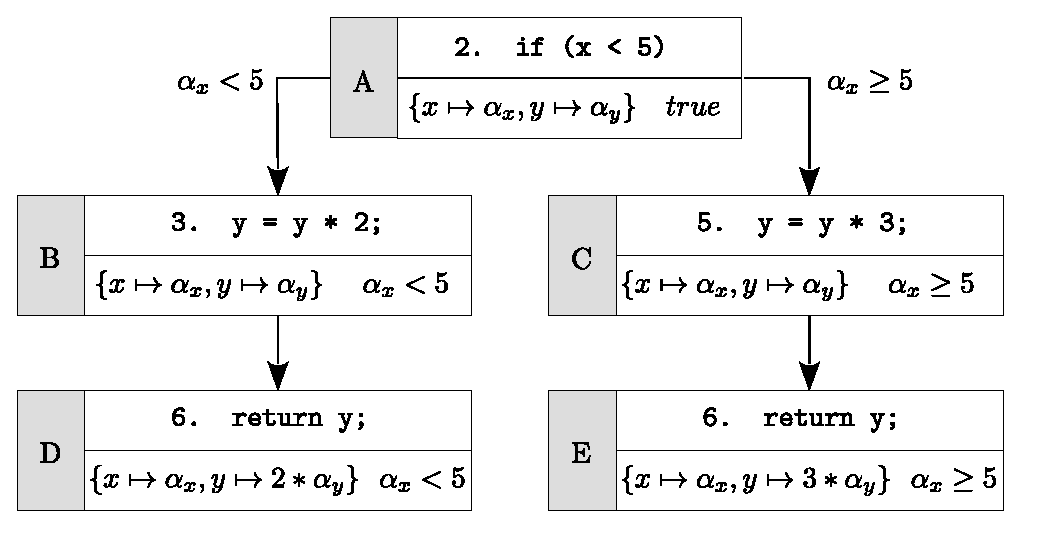
\includegraphics[width=1.05\columnwidth]{images/state-merging} 
    %\label{fig:sub1}
    \vspace{-6.5mm}
    \caption{}
  \end{subfigure}%
  \begin{subfigure}{.5\textwidth}
    \centering
    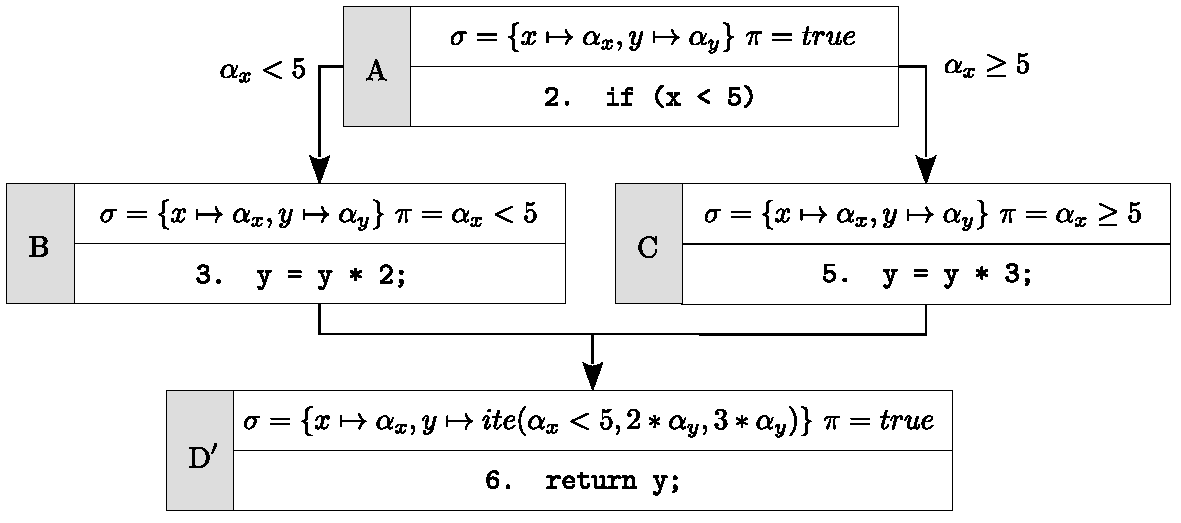
\includegraphics[width=1.05\columnwidth]{images/state-merging-2} 
    %\label{fig:sub2}
    \vspace{-4mm}
    \caption{}
  \end{subfigure}
  \vspace{-3mm}
  \caption{Symbolic execution of function \texttt{foo} of Figure~\ref{fi:example-state-merging}: (a) without state merging; (b) with state merging.}
  \label{fig:example-state-merging}
\end{figure}

%\vspace{-4pt} % TODO
\myparagraphnoperiod{Trade-Offs: to Merge or Not to Merge?} Early works~\cite{G-POPL07,HSS-RV09} have shown that merging techniques effectively decrease the number of paths to explore, but also put a burden on constraints solvers, which typically encounter difficulties when dealing with disjunction. Merging can also introduce new symbolic expressions in the code, for instance when merging different concrete values from a conditional assignment into a symbolic expression over the condition. \cite{KKB-PLDI12} provides an excellent discussion of the design space of state merging techniques. At the one end of the spectrum, complete separation of the paths does not perform any merge and is used in search-based symbolic execution (Section~\ref{ss:heuristics}). At the other end, static state merging combines states at control-flow join points, thus essentially representing a whole program with a single formula. Static state merging is used in whole-program verification condition generators\iffullver{, e.g.,} ~\cite{SATURN-POPL05,CALYSTO-ICSE08}), \iffullver{which typically trade precision for scalability by, for instance, unrolling loops only once.}{which usually trade precision for scalability by, e.g., unrolling loops only once.}

%At the other end, static state merging combines states at control-flow join points after all subpaths leading to a join point have been explored.

%\mynote{Function summaries}

\myparagraph{Merging Heuristics} Intermediate merging solutions adopt heuristics to identify state merges that can speed the exploration process up. Indeed, generating larger symbolic expressions and possibly extra solvers invocations can outweigh the benefit of having fewer states, leading to poorer overall performance~\cite{HSS-RV09,KKB-PLDI12}. {\em Query count estimation}~\cite{KKB-PLDI12} relies on a simple static analysis to identify how often each variable is used in branch conditions past any given point in the CFG. The estimate is used as a proxy for the number of solver queries that a given variable is likely to be part of. Two states make a good candidate for merging when their differing variables are expected to appear infrequently in later queries. {\em Veritesting}~\cite{VERITESTING-ICSE14} implements a form of merging heuristic based on a distinction between easy and hard statements. Hard statements are those that involve indirect jumps, system calls, and other operations for which precise static analyses are difficult to achieve. Static merging is performed on sequences of easy statements, %which are represented as a single path 
whose effects are captured using $ite$ expressions, 
while per-path symbolic exploration is done whenever a hard-to-analyze statement is encountered. 

%identifies sequences of statements that do not contain system calls, indirect jumps, and other statements that are difficult to reason about statically, and represents them with a single formula as in static state merging. The approach is alternated with a per-path basis symbolic exploration every time a hard-to-analyze statement is encountered. 

\myparagraph{Dynamic State Merging} Ideally, in order to maximize the opportunities for merging, a symbolic execution engine should traverse a CFG so that a combined state for a program point can be computed from its predecessors, e.g., if the graph is acyclic, by following a topological ordering. However, this would prevent search exploration strategies aiming at prioritizing more ``interesting'' states over others. \cite{KKB-PLDI12} introduces {\em dynamic state merging} to identify opportunities for merging regardless of the exploration order imposed by the search strategy.
Suppose the symbolic engine maintains a worklist of states and a bounded history of their predecessors. When the engine has to pick the next state to explore, it first checks whether there are two states $s_1$ and $s_2$ from the worklist such that they do not match for merging, but $s_1$ and a predecessor of $s_2$ do. If the expected similarity between $s_2$ and a successor of $s_1$ is also high, the algorithm attempts a merge by advancing the execution of $s_1$ for a fixed number of steps. This captures the idea that if two states are similar, then also their respective successors are likely to become similar in a few steps. If the merge fails, the algorithm lets the search heuristic pick the next state to explore.

%This is useful, for instance, for unbounded loops for which search-based symbolic execution engines would employ search strategies that prioritize exploring new code over unrolling, while static state merging would require a depth-first exploration and thus fully unroll the possibly infinitely many iterations of the loop.

% ---------------------------------------------------------------------------------------------------
\subsection{Leveraging Program Analysis and Optimization Techniques}
\label{ss:program-analysis}

A deeper understanding of a program's behavior can help a symbolic engine to focus on promising states, e.g., by pruning uninteresting parts of the computation tree. Several classical program analysis techniques have been explored in the symbolic execution literature. Some prominent examples are listed below:

\begin{itemize}

\item {\em Program slicing} is a method that, starting from a subset of a program's behavior, extracts from the program the minimal sequence of instructions that faithfully represents that behavior~\cite{Weiser84}. This information can help a symbolic engine in several ways: for instance, given a program slice related to a target program point, symbolic exploration can be restricted to paths contained in the program slice. We discuss an example of use in Section~\ref{ss:auth-bypass}.

\item {\em Taint analysis} attempts to check which variables of a program may hold values derived from potentially dangerous external sources such as user input. The analysis can be performed both statically and dynamically, with the latter yielding more accurate results. In the context of symbolic execution, taint analysis can help an engine skip execution paths that do not depend upon tainted values, effectively reducing the exploration state space~\cite{SAB-SP10}.

\item {\em Fuzzing} is a software testing technique that randomly mutates user-provided test inputs to cause crashes or assertion failures and find potential memory leaks. Fuzzing, as discussed in Section~\ref{ss:heuristics}, can be augmented with symbolic execution to collect constraints for an input and negate them to generate new inputs. On the other hand, a symbolic executor can be augmented with fuzzing to reach deeper states in the exploration more quickly and efficiently: we present two embodiments of this approach in Section~\ref{ss:bug-detection}.
  %\mynote{C: crossref: dynamic test generation}
  %\footnote{\cite{DRILLER-NDSS16} classifies offline symbolic executors such as {\sc DART} and {\sc SAGE} as {\em whitebox fuzzers}.}

\item {\em Branch predication} is a strategy for mitigating misprediction penalties in pipelined executions by avoiding jumps over very small sections of code: for instance, control-flow forking constructs such as the C ternary operator can be replaced with a predicated {\tt select} instruction. \cite{CCK-EUROSYS11} reports an exponential decrease in the number of paths to explore from the adoption of this strategy when cross-checking two implementations of a program using symbolic execution. % [D] alternative formulation: ~\cite{CCK-EUROSYS11} cross-checks two implementations of a program using symbolic execution and reports an exponential decrease in the number of paths to explore from the adoption of a simple form of this strategy; 
%  \item {\em source code analysis}: \mynote{TODO/drop?} extraction of input properties (e.g., size or contents of an array);

  \item {\em Type checking} can be effectively mixed with symbolic analysis~\cite{KCF-PLDI10};  for instance, type checking can determine the return type of a function that is difficult to analyze symbolically: such information can then potentially be used by the executor to prune certain paths\footnote{Interestingly,~\cite{KCF-PLDI10} discusses also how symbolic analysis can help a type checker. For instance, a symbolic engine can provide context-sensitive properties over a variable that would rule out certain type errors, improving the precision of the type checker.}.

  \item {\em State matching} determines whether an abstract state is subsumed by another, and can be used to analyze an under-approximation of a program's behavior. For instance, \cite{APV-SPIN06,VPP-ISSTA06} explore different heap shapes in the context of test generation for data structures, using subsumption checking to determine whether a symbolic state is being revisited. % ~\cite{XGM-ISSTA08} implements a different form of under-approximation: it looks for buffer overflows by having only a prefix of a buffer handled symbolically, and a symbolic length that may exceed the lenght of the prefix (any byte beyond the prefix is filled with concrete random data) - [D] I'm dropping this for now as we would have to call the item 'under-approximation' and change the first part of the text

\end{itemize}

\mytempedit{
\myparagraph{Classic Compiler Optimizations}
It has been also argued that program optimization techniques should be a first-class ingredient of practical implementations of symbolic execution, alongside widely accepted solutions such as search heuristics, state merging, and constraint solving optimizations~\cite{Cadar-FSE15}. In fact, program transformations can affect both the complexity of the constraints generated during path exploration and the exploration itself. For instance, precomputing the results of a function using a lookup table leads to a larger number of constraints in the path conditions due to memory accesses, while applying strength reduction for a multiplication by a constant results in a chain of addition operations that is more expensive for a constraint solver. Also, the way high-level {\tt switch} statements are compiled can significantly affect the performance of path exploration, while resorting to conditional instructions such as {\tt select} in LLVM or {\tt setcc} and {\tt cmov} in x86 can avoid expensive state forking by yielding {\em ite} expressions instead.

% D-THESIS14 superseded by DOZ-ISSRE15
%and none of them has tackled the analysis of binary programs.
While the effects of a compiler optimization can usually be predicted on the number or size of the instructions executed at run time, a similar reduction is not obvious in symbolic execution~\cite{DOZ-ISSRE15}, mostly because the constraint solver is typically used as a black-box. To the best of our knowledge, only a few works have attempted to analyze the impact of compiler optimizations on constraint generation and path exploration~\cite{WKC-HOTOS13,DOZ-ISSRE15}, leaving interesting open questions. \mynote{TODO: Move to 3.1?}Of a different flavor is the work presented in~\cite{PMZ-ISSTA17}, which explores transformations such as dynamic constant folding and optimized constraint encoding to speed up memory operations in symbolic executors based on theories of arrays (Section~\ref{ss:fully-symbolic-memory}).

\myparagraph{Further Directions}
We believe that the symbolic execution practice might also benefit from solutions that have been proposed for related problems in the program analysis realm. For instance, in the parallel computing community transformations such as {\em loop coalescing}~\cite{BGS-CSUR94} can restructure nested loops into a single loop by flattening the iteration space of their indexes. Such a transformation could potentially simplify a symbolic exploration, empowering search heuristics and state merging strategies. {\em Loop unfolding}~\cite{SK-SIGPLAN-NOTICES04} is another potentially interesting technique, as it allows exposing ``well-structured'' loops (e.g., showing invariant code, or having constants or affine functions as subscripts of array references) after peeling several iterations. {\em Program synthesis}~\cite{PR-POPL89} is a technique for automatic construction of a program satisfying a high-level specification, and in recent years has caught the attention of the verification community since it has been show how to find programs as a solution to SAT problems~\cite{Solar-Lezama08}. As we discussed in Section~\ref{se:environment-thirdparty}, \cite{JQF-ICSE16} has shown that program synthesis can be used to build models for complex Java components by abstracting away the details and entanglements of their implementations while capturing their functional behavior. In particular, the technique produces compact models by taking as inputs classes, methods and types from the framework, along with tutorial programs (typically those provided by the vendor) that exercise its parts. We believe this approach deserves further investigation in the context of the path explosion problem, as it could potentially be applied to software modules such as standard libraries to produce concise models that allow for a more scalable exploration of the search space. 
}

   %%%% DROPPED PARTS
    %\item {\em compositional techniques}: caching and reusing the analysis of lower-level function in subsequent computations. The main idea is to compute function summaries. See, e.g.,~\cite{G-POPL07,G-PLDI11,MS-TR07}.
   %%%% REWRITTEN PARTS
  %\item {\em phi-node folding} is a code transformation that can be used for statically merging some paths\mynote{E: relation with state merging?}. The main idea is to replace branches with predicated select instructions. Using this technique, the number of paths that must be explored by a symbolic engine can be significantly decreased. For instance,~\cite{CCK-EUROSYS11} used an aggressive variant of phi-node folding, called {\em if-conversion}~\cite{CCF-CGO03}, that allowed them to reduce the number of paths by an exponential factor on some benchmarks.
%\item \cite{DRILLER-NDSS16} is an example of {\em symbolic-assisted fuzzing}: their technique temporarily exploits concolic execution only when a fuzzer cannot generate a valid input to explore an uncovered branch.
 % \item {\em abstraction}~\cite{C-SEFM07} is a technique that may be used for computing {\em under-approximations} or {\em over-approximations} of a program state. This approach has been exploited in prior works~\cite{APV-SPIN06,VPP-ISSTA06,XGM-ISSTA08}\mynote{check these papers}. Since some of these works reason about state subsumption, they may be connected with the incremental solving optimization discussed in Section~\ref{constraint-optimizations}.
   %\item {\em type-checking}: \cite{KCF-PLDI10} shows how symbolic analysis can be effectively mixed with type-checking analysis. For instance, type-checking analysis can help a symbolic execution engine by detecting the type of an object (e.g., the type of a value returned by a {\em hard to reason} function). Although no assumption can be made on the value of the returned type, this information may still be useful for the symbolic engine (e.g., if the type has a fixed size, some preconditions can be set, possibly pruning some paths). Similarly, symbolic analysis can help a type checker. For instance, the symbolic engine may provide context-sensitive properties over a variable that clearly rules out type errors, reducing the number of false positive given by a traditional context-insensitive type checker.
